\documentclass{article}
\usepackage{amsmath}
\usepackage{amssymb}
\usepackage{graphicx}
\usepackage{hyperref}
\usepackage[version=4]{mhchem}


\begin{document}
In \(\triangle A B C\), the angle bisectors of \(\angle B, \angle C\) meet at \(T\), and the exterior angle bisectors of \(\angle B, \angle C\) meet at \(P\). Show that\\
\(\angle B P C=\frac{1}{2}(\angle A B C+\angle A C B)\).

Solution:
Label \(\angle T B C=\angle T B A=\alpha, \angle T C B=\angle T C A=\beta, \angle C B P=\)\\
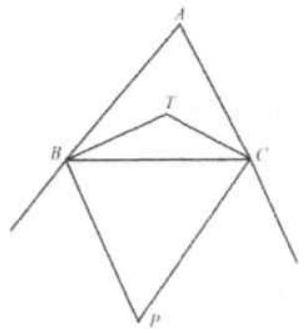
\includegraphics[width=\textwidth]{images/195.jpg} \(\gamma\).\\
Since \(2 \alpha+2 \gamma=180^{\circ}, \alpha+\gamma=90^{\circ}\).\\
Thus \(\angle T B P=90^{\circ}\).\\
Similarly, \(\angle T C P=90^{\circ}\).\\
So points \(B, P, C\), and \(T\) are concyclic and \(T P\) is the diameter of the circle.\\
Therefore, \(\angle B P T=\angle T C B=\beta, \angle C P T=\angle T B C=\alpha\).\\
\centering
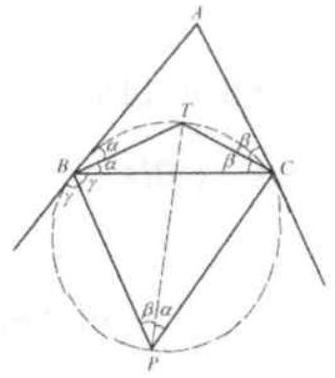
\includegraphics[width=\textwidth]{images/195(1).jpg}\\
\(\angle B P C=\alpha+\beta=\angle T B C+\angle T C B\)\\
\(=\frac{1}{2}(\angle A B C+\angle A C B)\).



\end{document}
